\chapter{Definitions}

\section{Simple hypergraphs}

\begin{defn}
	Hypergraph is a tuple $(X, \M)$ where $\M \subseteq \mathcal{P}(X)$. Or generally just a set system.
\end{defn}

\begin{defn}
	A simple hypergraph (linear, $k$-graph) is $(X,\M)$ if $M_1 \neq M_2 \in \M \Rightarrow |M_1 \cap M_2| \leq 1$.
\end{defn}

\begin{example}
	Lets see some of the easier examples of simple hypergraphs.
	
	\begin{itemize}
		\item Graphs themselves are simple hypergraphs. Where $(X, \M)$ and $\M \subseteq \binom{X}{2}$.
		\item Or generally $k$-graphs, where $\M \subseteq \binom{X}{k}$.
		\item A well known Fano plane, see picture \ref{fano-plane}.
		\item Lets have a set of points $A$ and define $X = \binom{A}{2}$; which are edges in $A$ and $\M = \{\binom{T}{2} | |T| = 3, T \subseteq A\}$; which are triangles in $A$. This is also simple.
	\end{itemize}
\end{example}


\begin{defn}
	A chromatic number of such hypergraphs is defined in a following way:
	
	$$
	\chi (X,\M) := \min \{k | \exists \bigcup_{i=1}^k X_i = X \text{ and no } X_i \text{ contains } M \in \M\}.
	$$
\end{defn}

\noindent In other words: At least two "colors" for each $M \in \M$. And by Ramsey theory we may state that $\forall k \ \exists X: \chi(X,\M) > k$.

\begin{example}
	For fixed $k \in \N$ we have $k$ committees, each of them has $k$ members and they are meeting in a room with $k$ seats. Any two committees are disjoint. Can someone sit at the same place? And how many of them? -- This was stated by Erd\H os, Faber and Lovász in 1972.
\end{example}

\begin{thm}[Kuhn, Osthus, Kang, Kelly, Methuku, 2023]
	Showed that the previous example is true for large $k$.
\end{thm}

A different formulation can be said using simple hypergraphs. Lets have simple hypergraf $(X,\M)$ where $|\M| = k$ and line chromatic number $\leq k$. That is coloring the edges instead. If they meet they have to be distinct.

\begin{prop}
	$\chi_l (K_{2k}) = 2k-1$ for $k \in \N$.
\end{prop}

\begin{proof}[Sketch of proof]
	Lets draw the graph, so the vertices are on a circle. Then take the edges across in the same direction and one from the inside of the circle to the boundary and color them. Then rotate and color once again, until colored.
\end{proof}

\section{Dual hypergraphs}

Lets now define a dual hypergraphs, which may not be so intuitive at a first glance. Lets see a picture \ref{dual-hg} showing the incidence graph for $(X,\M)$. Then the dual is obtained by switching the parts of $(X, \M)$ and $(\M',X')$. Lets denote the dual of $(X,\M)$ as $d(X,\M)$.

\begin{figure}[!ht]\centering
	\begin{subfigure}{.45\textwidth}
		\begin{tikzpicture}
			\draw (0,0) to (6,0);
			\draw (0,3) to (6,3);
			\node (X) at (6.5,0) {$\M$};
			\node (M) at (6.5,3) {$X$};
			\draw (2,0) -- (1,3) node[midway, below, left] {$\in$};
			\draw (2,0) -- (2,3);
			\draw (2,0) -- (3,3);
			\draw (2,0) -- (4,3);
			\node (M) at (2,-.2) {$M$};
			\node (x1) at (1,3.2) {$x_1$};
			\node (x2) at (2,3.2) {$x_2$};
			\node (x3) at (3,3.2) {$x_3$};
			\node (x4) at (4,3.2) {$x_4$};
		\end{tikzpicture}
	\end{subfigure}
	\begin{subfigure}{.45\textwidth}
		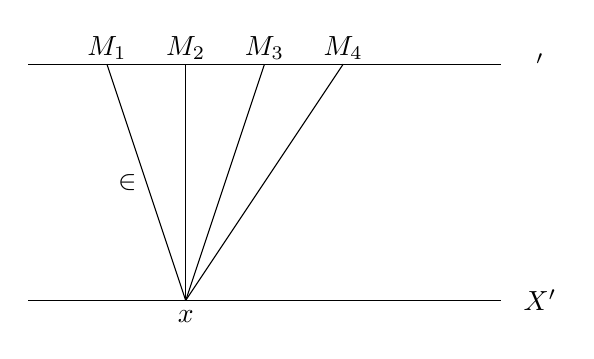
\begin{tikzpicture}
			\draw (0,0) to (6,0);
			\draw (0,3) to (6,3);
			\node (X) at (6.5,0) {$X'$};
			\node (M) at (6.5,3) {$\M'$};
			\draw (2,0) -- (1,3) node[midway, below, left] {$\in$};
			\draw (2,0) -- (2,3);
			\draw (2,0) -- (3,3);
			\draw (2,0) -- (4,3);
			\node (M) at (2,-.2) {$x$};
			\node (x1) at (1,3.2) {$M_1$};
			\node (x2) at (2,3.2) {$M_2$};
			\node (x3) at (3,3.2) {$M_3$};
			\node (x4) at (4,3.2) {$M_4$};
		\end{tikzpicture}
	\end{subfigure}
	\caption{Diagram for the dual hypergraph.}
	\label{dual-hg}
\end{figure}

\begin{lemma}
	$(X,\M)$ is simple \ifft $d(X,\M)$ is simple.
\end{lemma}

\begin{proof}[Proof by picture]
	For the proof see the picture \ref{simple-dual-hg}. This $C_4$ like structure happens if it is not simple and hence when we flip the diagram, obtaining the dual, the diagram does not change.
	
	\begin{figure}[!ht]\centering
		\begin{tikzpicture}
			\draw (0,0) to (6,0);
			\draw (0,3) to (6,3);
			\node (X) at (6.5,0) {$\M$};
			\node (M) at (6.5,3) {$X$};
			\draw (2,0) -- (2,3);
			\draw (4,0) -- (4,3);
			\draw (2,0) -- (4,3);
			\draw (4,0) -- (2,3);
			\node (M1) at (2,-.2) {$M_1$};
			\node (M2) at (4,-.2) {$M_2$};
			\node (x1) at (2,3.2) {$x_1$};
			\node (x2) at (4,3.2) {$x_2$};
		\end{tikzpicture}
		\caption{Simple dual graphs proof.}
		\label{simple-dual-hg}
	\end{figure}
\end{proof}

Now lets denote $A(X,\M)$ as an incidence matrix of a given hypergraph, then the dual has incidence matrix $A(d(X,\M)) = A^T(X,\M)$.

Lets consider $(X, \M)$ a $k$-uniform hypergraph. Can we somehow bound the size of $|\M|$? We may establish trivial bounds as $0 \leq |\M| \leq \binom{X}{k}$. We will further on make better bounds. Lets see the picture \ref{bounds}. We will be using double counting method, for which we notice that for some $\binom{X}{2}$ we have at least one $M \in \M$.

\begin{figure}[!ht]\centering
	\begin{tikzpicture}
		\draw (0,0) to (6,0);
		\draw (0,3) to (6,3);
		\node (X) at (6.5,0) {$\M$};
		\node (M) at (6.5,3) {$\binom{X}{2}$};
		\draw (4,0) -- (4,3);
		\draw (4,0) -- (3,3);
		\draw (4,0) -- (5,3);
		\node (M) at (4,-.2) {$M$};
		\node (Xo2) at (1,3.3) {$\binom{X}{2}$};
		\draw (1,3) -- (2,0);
		
		\node (x2) at (4,3.3) {$\binom{k}{2}$};
	\end{tikzpicture}
	\caption{Providing better bound.}
	\label{bounds}
\end{figure}

\noindent Hence we may compute the following.

$$
|\M| \cdot \binom{k}{2} = \sum_{M \in \M} \binom{|M|}{2} \leq \binom{|X|}{2}
$$

\noindent Therefore we can obtain the bound.

$$
|\M| \leq \frac{\binom{|X|}{2}}{\binom{k}{2}}
$$

\noindent See that this bound is actually tight. For $k=2$ we can consider a graph $K_n$ and for $k=3$ we may look at Fano plane. If the equality hold we call it \textit{Steiner system}. Or in other words it is true if $\forall x \neq y \in X \ \exists! M \in \M$ such that $\{x,y\} \subseteq M$. For $k = 3$ we call this \textit{Steiner triple system} or STS for short (one can be seen as Fano plane and the other as another seen on picture \ref{k=3}). This is particularly used in experiments and mainly in agriculture. Usually this is then denoted as \textit{BIBD} which stands for balanced incomplete block design.

\begin{figure}[!ht]\centering
	\begin{tikzpicture}[scale=.6, l/.style = {line width=2pt},
		n/.style = {draw, circle, fill, inner sep=1.5pt},
		o/.style = {myorange},
		r/.style = {myred},
		b/.style = {myblue},
		g/.style = {mygreen},
		p/.style = {myviolet}]
		\foreach \j in {1,...,3} {
			\foreach \i in {1,...,3} {
				\node[n] (\j-\i) at (2*\j,2*\i) {};
			}
		}
		
		\draw[l,o] (1-1) to (1-2) to (1-3);
		\draw[l,o] (2-1) to (2-2) to (2-3);
		\draw[l,o] (3-1) to (3-2) to (3-3);
		
		\draw[l,b] (1-1) to (2-1) to (3-1);
		\draw[l,b] (1-2) to (2-2) to (3-2);
		\draw[l,b] (1-3) to (2-3) to (3-3);
		
		\draw[l,g] (1-1) to (2-2) to (3-3);
		\draw[l,g] (1-2) to (2-3) to[out=20,in=180] (6.5,6.5) to[out=0, in=0] (3-1);
		\draw[l,g] (1-3) to[out=200,in=180] (1.5,1.5) to[out=0,in=200] (2-1) to (3-2);
		
		\draw[l,r] (1-1) to[out=330,in=250] (6.5,1.5) to[out=70,in=330] (3-2) to (2-3);
		\draw[l,r] (3-3) to[out=120,in=0] (1.5,6.5) to[out=180,in=150] (1-2) to (2-1);
		\draw[l,r] (1-3) to (2-2) to (3-1);
	\end{tikzpicture}
	\caption{Another Steiner triple system.}
	\label{k=3}
\end{figure}

We may say that for STS to exists it must hold that both $n-1$ and $\frac{\binom{n}{2}}{\binom{3}{2}}$ must be integers. So it only exists if $n$ is either $6k+1$ or $6k+3$.

\begin{thm}
	Steiner triple system exists \ifft $n$ is either $6k+1$ or $6k+3$.
\end{thm}

\begin{proof}
	We will be showing how it can be generated. That is from two STS we create a new one. First we can observe that if both $(X_1, \M_1)$ and $(X_2, \M_2)$ are STS then also $(X_1 \times X_2, \M)$ is STS, where $\M$ can be viewed from a picture \ref{M-def} or from an algebraic view. That is we have algebra of $(X, \M)$ $\mathbb{A}_{(X,\M)}$ then it is $\mathbb{A}_{(X_1,\M_1)} \times \mathbb{A}_{(X_2,\M_2)}$.
	
	\begin{figure}[!ht]\centering
		\begin{tikzpicture}[thick]
			\draw (1,1) -- (7,1);
			\draw (1,1) -- (1,7);
			\node at (6.6, 0.6) {$(X_2, \M_2)$};
			\node at (0, 6.6) {$(X_1, \M_1)$};
			\node[myblue] at (0.6, 2) {$x_1$};
			\node[myblue] at (0.6, 3) {$y_1$};
			\node[myblue] at (0.6, 5) {$z_1$};
			\node[mygreen] at (2, 0.6) {$x_2$};
			\node[mygreen] at (4, 0.6) {$y_2$};
			\node[mygreen] at (5, 0.6) {$z_2$};
			\node[myorange] at (2, 2) (x) {$x$};
			\node[myorange] at (4, 3) (y) {$y$};
			\node[myorange] at (5, 5) (z) {$z$};
			\draw (2,1) -- (x);
			\draw (1,2) -- (x);
			\draw (4,1) -- (y);
			\draw (1,3) -- (y);
			\draw (5,1) -- (z);
			\draw (1,5) -- (z);
		\end{tikzpicture}
		\caption{Definition of $\M$, where $\{x,y,z\} \in \M$.}
		\label{M-def}
	\end{figure}
\end{proof}

\section{Introducing BIBD and integrality conditions}

\begin{defn}[BIBD]
	Hypergraph $(X, \M)$ is BIBD with parameters $(v,k,\lambda,t)$ if $|X| = v$ $\M \subseteq \binom{X}{k}$ and $\forall x_1, \dots x_t \in \binom{X}{t}$ we have that $|\{M \in \M | \{x_1, \dots, x_t\} \subseteq M\}| = \lambda$. 
\end{defn}

With the similar arguments we may see that $|\M| = \frac{\binom{|X|}{t}}{\binom{k}{t}} \cdot \lambda$ this holds and hence it has to be an integer. Now the question is whether there actually exists BIBD with given values $(n,k,\lambda,t)$? There is pretty simple observation that if we take $A \subseteq X$ of size $|A| = a$ it must be true that $\frac{\binom{n - a}{t - a}}{\binom{k - a}{t - a}} \cdot \lambda$ must be integer for the number of such $M$'s containing $A$. From these properties we establish the integer constraints for the existence of BIBD.

\begin{prop}[BIBD necessary constraints]
	If we have BIBD $(n,k,\lambda,t)$ everything has to hold. Firstly the size of $\M$
	
	$$
	|\M| = \frac{\binom{|X|}{t}}{\binom{k}{t}} \cdot \lambda
	$$
	
	\noindent and also the integrality of the following fractions.
	
	$$
	\frac{\binom{n - a}{t - a}}{\binom{k - a}{t - a}} \cdot \lambda \ \text{for } a = 1, \dots, t.
	$$
\end{prop}

Now recall that we have shown how two STS can create a new STS. Now we will show a similar proposition.

\begin{prop}
	If there exists BIBD $(v,3,2,1)$ then also BIBD $(2v +1,3,2,1)$ exists.
\end{prop}

\begin{proof}
	The proof is by a picture \ref{new-sts-twice}. Firstly lets have STS and duplicate it. Then also add new vertex. We will create new $M$'s so that the properties of STS are still satisfied. Which also includes the newly created vertex.
	
	\begin{figure}[!ht]\centering
		\begin{tikzpicture}[main/.style = {circle, draw, fill, inner sep=1.5pt}]
			\node[main] at (8,-2) (c) {};
			\foreach \x in {1,...,7} {
				\node[main] at (2*\x, 1) (1-\x) {};
				\node[main] at (2*\x, 3) (2-\x) {};
				\path[draw, line width=1.5pt, myorange] (c) -- (1-\x) -- (2-\x);
			}
			\draw[myblue, fill, fill opacity=0.5] (1.5,3.5) rectangle (6.5,2.5);
			\node[myblue] at (1, 3) {$M_1$};
			\draw[mygreen, fill, fill opacity=0.5] (1.5,1.5) rectangle (6.5,0.5);
			\node[mygreen] at (1, 1) {$M_2$};
		\end{tikzpicture}
		\caption{Newly created larger STS, where for $M_1$ and $M_2$ we create all possible $M$ so that at least one element is from $M_1$ and $M_2$ and in total we have 3 elements.}
		\label{new-sts-twice}
	\end{figure}
\end{proof}

\begin{thm}[R. Wilson, R. Chatouri]
	$\forall k, \lambda, t =2$ for every large $n$ the integrality conditions are sufficient for the existence of BIBD.
\end{thm}